\documentclass{article}
\usepackage{ben-basic}
\title{Effective Text Editing}
\begin{document}
\pdfbookmark[section]{Contents}{toc}
%\shorttoc{Contents}{1}
\tableofcontents
\clearpage

\section{Git}
\subsection{Authentication Method Ranking}
There are three main options for establishing authentication for write actions like a "push" with a Git.  My criteria for considering both security and productivity results in the following preference order: SSH, password access tokens, password client managers.  SSH is always my first choice, because it offers great convenience and high security standards with the use of the latest RSA public-key encryption.  Yet, some network environments may not allow SSH throughput, therefore "password access tokens" can be used against HTTPS with minimal effort.  As far as password manager clients, it nearly goes without saying that the cumbersome aspect of installing more software to config and set up is not compelling, although, it may offer better security of HTTPS if your current file system is secure.
\subsubsection{SSH}

\subsubsection{Password Access Tokens}

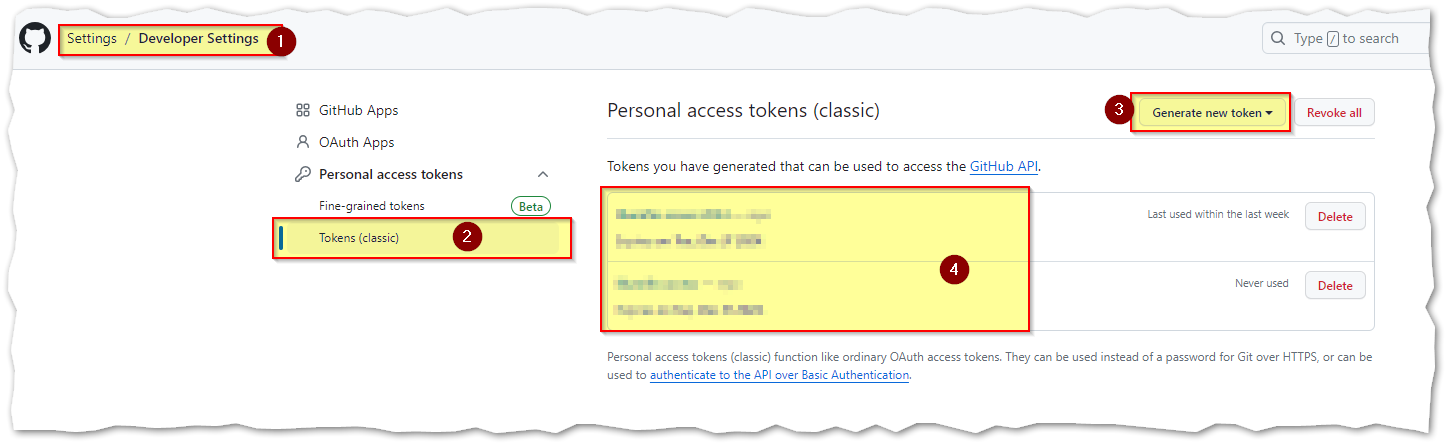
\includegraphics[width=200px]{images/Personal-Access-Tokens.png}
git config credential.helper 'store [<options>]'
\end{document}
